\documentclass[thesis]{subfiles}

\begin{document}

\chapter{Testy}

Aplikacje wykorzystujące do~działania komunikację sieciową wymagają szczególnie dokładnych testów --- z~natury działania komunikacji sieciowej wynika bowiem wiele zazwyczaj niespodziewanych sytuacji, które aplikacja musi umieć obsłużyć, np.~opóźnienia w~działaniu sieci czy nagłe zerwanie połączenia sieciowego, np.~na~skutek odłączenia kabla ethernetowego lub~wyłączenia przełącznika sieciowego, do~którego podłączona jest maszyna kliencka --- to~tylko niektóre z~sytuacji, z~którymi każdy protokół i~aplikacja sieciowa muszą sobie umieć poradzić.

Niniejszy rozdział opisuje testy funkcjonalne części serwerowej i~klienckiej stworzonej aplikacji.

%------------------------------------------------------------------------------
%
%\section{Monitorowanie wykorzystania zasobów}
%
%\noindent Poniżej przedstawiono testy użycia zasobów, takich jak:
%\begin{itemize}
%	\item pamięci,
%	\item plików,
%	\item \glslink{socket}{socketów},
%	\item \gls{fifo} (potok nazwany).
%\end{itemize}
%
%------------------------------------------------------------------------------

\section{Testy funkcjonalne}

Przeprowadzone testy wykonano w~środowisku złożonym z~trzech fizycznych komputerów klasy~PC z~zainstalowanym systemem \emph{Linux Debian} oraz~dwóch maszyn wirtualnych \hrefemph{https://www.virtualbox.org/}{VirtualBox~5.1} z~zainstalowanym systemem \emph{Linux Arch}. Jeden z~komputerów z~zainstalowanym systemem \emph{Linux Debian} odgrywa rolę serwera i~klienta, a~pozostałe komputery są~klientami. Schemat testowej sieci został przedstawiony na rysunku~\ref{fig:testing-network}.

\begin{figure}
	\centering
	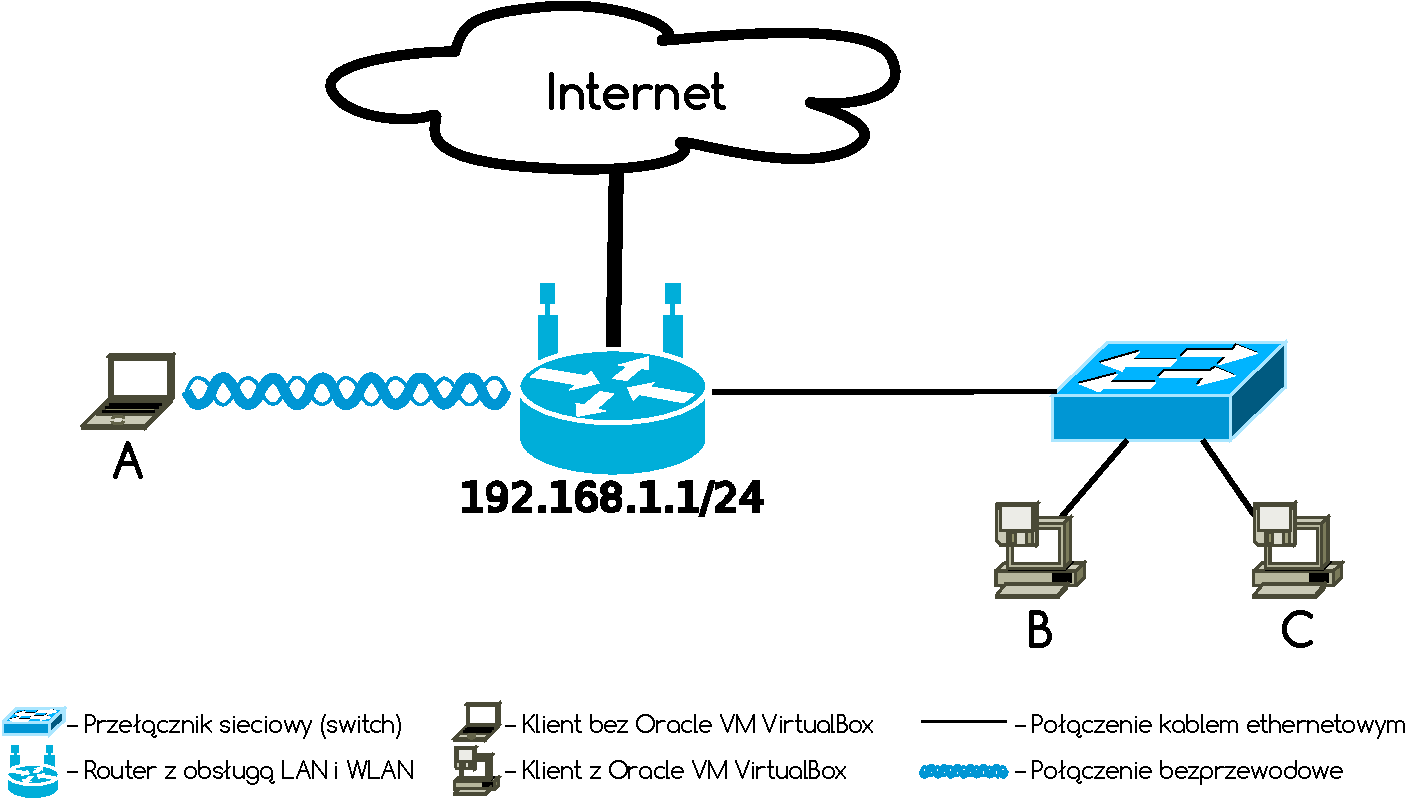
\includegraphics[width=0.8\textwidth]{img/testing-network}
	\caption{Schemat przedstawiający konfigurację sieciową środowiska testowego}
	\label{fig:testing-network}
\end{figure}

TODO

\end{document}
